\section{Nuclear Reactions}
\subsection{Mass Excess}
\[ \Delta_\text{Atom} = \text{Z} \times \text{M}_\text{Proton} + (\text{A-Z}) \times \text{M}_\text{Neutron} - \text{M}_\text{Atom}
\]
\subsection{Energy Released}
$ a + b \rightarrow c + d$ or $a(b,c)d$ \\
$Q$, energy released, =
\[Q = [(M_a + M_b) - (M_c + M_d)] c^2\]
$Q > 0$ is exothermic, $Q < 0$ is endothermic

\subsection{Cross Sections}
Reaction Rate $R$, microscopic cross-section $\sigma$
\[ R~[\SI[per-mode=fraction]{}{\number\per\square\centi\metre\per\second}] = \sigma~[\SI[per-mode=fraction]{}{\square\centi\metre}]~ I~[\SI[per-mode=fraction]{}{\number\per\square\centi\metre\per\second}]~ N_A~[\SI[per-mode=fraction]{}{\number\per\square\centi\metre}] \]
\[
R = \Sigma_T I \qquad \Sigma_T = N \sigma_T
\]

Beam $I$, macroscopic cross-section $\Sigma_T$
\begin{align*}
I(x) &= I_0 \exp{-\Sigma_T x} \\
\Sigma_T &= N_X \sigma^X_t + N_Y \sigma^Y_t + N_Z \sigma^Z_t + \ldots = \frac{1}{\lambda}
\end{align*}
$\lambda = $ Mean free path (until 1\textsuperscript{st} interaction)
$\nu~\Sigma_T = [\SI{}{\per\second}]$ Collision Freq., $\nu = $ neutron speed

\subsubsection{Neutron Cross Section Hierarchy}
\resizebox{\linewidth}{!}{%
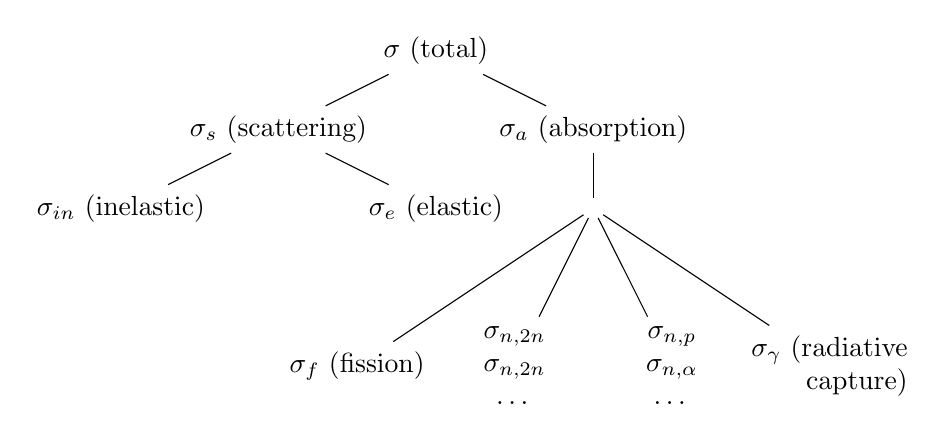
\begin{tikzpicture}
\node (v1) at (0,3) {$\sigma$ (total)};
\node (v2) at (-2,2) {$\sigma_s$ (scattering)};
\node (v3) at (2,2) {$\sigma_a$ (absorption)};
\draw  (v1) edge (v2);
\draw  (v1) edge (v3);
\node (v5) at (0,1) {$\sigma_e$ (elastic)};
\node (v4) at (-4,1) {$\sigma_{in}$ (inelastic)};
\draw  (v2) edge (v4);
\draw  (v2) edge (v5);
\node (v6) at (2,1) {};
\draw  (v3) edge (v6);
\node (v7) at (-1,-1) {$\sigma_f$ (fission)};
\node [align=center] (v8) at (1,-1) {$\sigma_{n,2n}$ \\ $\sigma_{n,2n}$ \\ \ldots};
\node [align=center] (v9) at (3,-1) {$\sigma_{n,p}$ \\ $\sigma_{n,\alpha}$ \\ \ldots};
\node [align=right] (v10) at (5,-1) {$\sigma_\gamma$ (radiative \\ capture)};
\draw  (v6) edge (v7);
\draw  (v6) edge (v8);
\draw  (v6) edge (v9);
\draw  (v6) edge (v10);
\end{tikzpicture}
}
